
% This LaTeX was auto-generated from MATLAB code.
% To make changes, update the MATLAB code and republish this document.

\documentclass{article}
\usepackage{graphicx}
\usepackage{color}

\sloppy
\definecolor{lightgray}{gray}{0.5}
\setlength{\parindent}{0pt}

\begin{document}

    
    
\section*{Infinite Impulse Response Filter Design}

\begin{par}
This code will prove to be classic example for proper use of the given functions for Butterworth filter, Chebyshev Type 1 filter and Chebyshev Type 2 Filter Design
\end{par} \vspace{1em}

\subsection*{Contents}

\begin{itemize}
\setlength{\itemsep}{-1ex}
   \item Inputs Provided
   \item Derivation of order by butterord
   \item Formula for Order n of Butterworth filter
   \item Applying the Butterworth filter function
   \item Converting to frequency domain.
   \item The PLOT for Butterworth Filter
   \item Butterworth Filter Characteristics
   \item Butterworth Filter Characteristics
   \item Derivation of order
   \item Applying the Chebyshev Type I filter function
   \item Converting to frequency domain.
   \item The PLOT for Chebyshev Type I Filter
   \item Derivation of order
   \item Applying the Chebyshev Type II filter function
   \item Converting to frequency domain.
   \item The PLOT for Chebyshev Type II Filter
   \item Author: Kaustubh Shivdikar
\end{itemize}


\subsection*{Inputs Provided}

\begin{par}
Passband Attenuation
\end{par} \vspace{1em}
\begin{verbatim}
Ap = 3;
\end{verbatim}
\begin{par}
Sampling Frequency
\end{par} \vspace{1em}
\begin{verbatim}
Fs = 500;
\end{verbatim}
\begin{par}
Stopband Attenuation
\end{par} \vspace{1em}
\begin{verbatim}
As = 60;
\end{verbatim}
\begin{par}
Passband Frequency
\end{par} \vspace{1em}
\begin{verbatim}
Wp = 40;
\end{verbatim}
\begin{par}
Dividing by Sampling Frequeny
\end{par} \vspace{1em}
\begin{verbatim}
Wp = Wp / Fs;
\end{verbatim}
\begin{par}
Stopband Frequency
\end{par} \vspace{1em}
\begin{verbatim}
Ws = 150;
\end{verbatim}
\begin{par}
Dividing by Sampling Frequeny
\end{par} \vspace{1em}
\begin{verbatim}
Ws = Ws / Fs;
\end{verbatim}


\subsection*{Derivation of order by butterord}

\begin{verbatim}
[n,Wn] = buttord(Wp,Ws,Ap,As);
\end{verbatim}


\subsection*{Formula for Order n of Butterworth filter}

\begin{par}

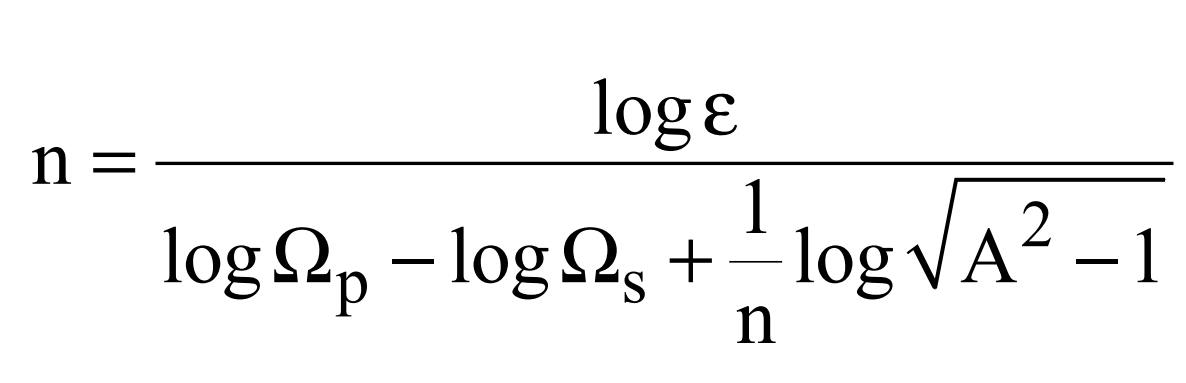
\includegraphics [width=4in]{D:\Github Live\Infinite-Impulse-Response-Filters\Source\f6.png}

\end{par} \vspace{1em}
\begin{par}
OR another simplified version will be
\end{par} \vspace{1em}
\begin{par}

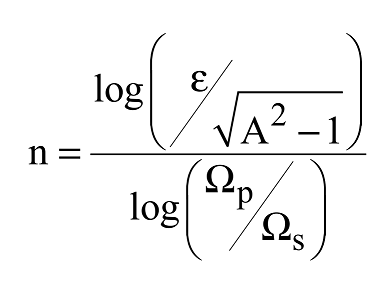
\includegraphics [width=4in]{D:\Github Live\Infinite-Impulse-Response-Filters\Source\f5.png}

\end{par} \vspace{1em}


\subsection*{Applying the Butterworth filter function}

\begin{verbatim}
[b,a] = butter(n,Wn);
\end{verbatim}


\subsection*{Converting to frequency domain.}

\begin{verbatim}
[h,w] = freqz(b,a);
\end{verbatim}
\begin{par}
Since the obtained input was in Normalized Form we get it back by multiplying with Sampling Frequency
\end{par} \vspace{1em}
\begin{verbatim}
W = w*Fs/pi;
\end{verbatim}
\begin{par}
To remove the negative values of h we take absolute
\end{par} \vspace{1em}
\begin{verbatim}
h = abs(h);
\end{verbatim}


\subsection*{The PLOT for Butterworth Filter}

\begin{verbatim}
figure();
plot(W,h);
title('Butterworth Filter')
\end{verbatim}

\includegraphics [width=4in]{IIR_01.eps}


\subsection*{Butterworth Filter Characteristics}

\begin{par}

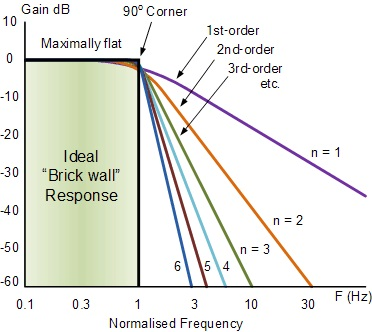
\includegraphics [width=4in]{D:\Github Live\Infinite-Impulse-Response-Filters\Source\graph1.gif}

\end{par} \vspace{1em}


\subsection*{Butterworth Filter Characteristics}

\begin{par}

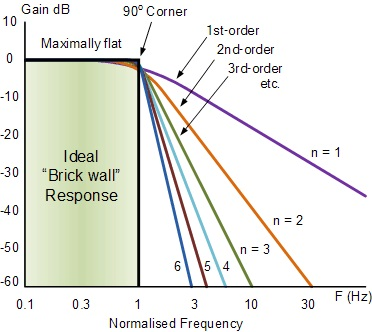
\includegraphics [width=4in]{D:\Github Live\Infinite-Impulse-Response-Filters\Source\graph1.gif}

\end{par} \vspace{1em}


\subsection*{Derivation of order}

\begin{verbatim}
[n,Wp] = cheb1ord(Wp,Ws,Ap,As);
\end{verbatim}


\subsection*{Applying the Chebyshev Type I filter function}

\begin{verbatim}
[b,a] = cheby1(n,Ap,Wp);
\end{verbatim}


\subsection*{Converting to frequency domain.}

\begin{verbatim}
[h,w] = freqz(b,a);
\end{verbatim}
\begin{par}
Again since the obtained input was in Normalized Form we get it back by multiplying with Sampling Frequency
\end{par} \vspace{1em}
\begin{verbatim}
W = w*Fs/pi;
\end{verbatim}
\begin{par}
Again to remove the negative values of h we take absolute
\end{par} \vspace{1em}
\begin{verbatim}
h = abs(h);
\end{verbatim}


\subsection*{The PLOT for Chebyshev Type I Filter}

\begin{verbatim}
figure();
plot(W,h);
title('Chebyshev Type I Lowpass Filter')
\end{verbatim}

\includegraphics [width=4in]{IIR_02.eps}


\subsection*{Derivation of order}

\begin{verbatim}
[n,Wp] = cheb2ord(Wp,Ws,Ap,As);
\end{verbatim}


\subsection*{Applying the Chebyshev Type II filter function}

\begin{verbatim}
[b,a] = cheby2(n,As,Wp);
\end{verbatim}


\subsection*{Converting to frequency domain.}

\begin{verbatim}
[h,w] = freqz(b,a);
\end{verbatim}
\begin{par}
Again since the obtained input was in Normalized Form we get it back by multiplying with Sampling Frequency
\end{par} \vspace{1em}
\begin{verbatim}
W = w*Fs/pi;
\end{verbatim}
\begin{par}
Again to remove the negative values of h we take absolute
\end{par} \vspace{1em}
\begin{verbatim}
h = abs(h);
\end{verbatim}


\subsection*{The PLOT for Chebyshev Type II Filter}

\begin{verbatim}
figure();
plot(W,h);
title('Chebyshev Type II Lowpass Filter')
\end{verbatim}

\includegraphics [width=4in]{IIR_03.eps}


\subsection*{Author: Kaustubh Shivdikar}

\begin{par}
MATLAB Lab experiment of Linear to circular convolution.
\end{par} \vspace{1em}
\begin{par}


\includegraphics [width=4in]{D:\Github Live\Infinite-Impulse-Response-Filters\Source\matlablogo.png}

\end{par} \vspace{1em}



\end{document}
    
